\documentclass{article}

\usepackage{fullpage}
\usepackage{amsmath}
\usepackage{graphicx}
\usepackage{tabu}
\usepackage{multirow}

\begin{document}

\title{Use of a Smoothed Heaviside Step Function \\ for the Arithmetic-Mean Average Type\footnote{The arithmetic-mean average type currently implemented in the codes corresponds to \texttt{avg\_type=7} in this report. Please read first the preceding report (\texttt{repo1} in the same directory). Note that based on the results present in these two reports the current version of \texttt{avg\_type=1} has been implemented.}~\footnote{For the actual run script, inputs file, and post-processing scripts, see \texttt{exec/reactDiff/test/misc/Schlogl\_hist\_1d}.}}

\date{}

\maketitle

\section{Motivation}

It has been observed that the following arithmetic-mean average type for the spatial discretization of the stochastic flux exhibits favorable behaviors on the cell number density distribution $\rho(n)$ and the structure factor $S(k)$:
\begin{equation}
\tilde{n}_\mathrm{arith}=
\begin{cases} 
\frac12(n_1+n_2) & \mbox{if $n_1\ge0$ and $n_2\ge0$,} \\ 
0 & \mbox{otherwise.}
\end{cases}
\end{equation}
As a function of $(n_1,n_2)$, this has a discontinuity, which can be seen through the following equivalent representation with the Heaviside step function $H(x)$:
\begin{equation}
\tilde{n}_\mathrm{arith} = \frac{1}{2}(n_1+n_2)H(\mathrm{min}(n_1,n_2)).
\end{equation}

In this report, $H(x)$ is replaced by some smoothed Heaviside step functions and the resulting changes in $\rho(n)$ and $S(k)$ are investigated.

\section{Arithmetic-Mean Average Type with a Smoothed Heaviside Step Function} 

\begin{figure}[t]
\centering
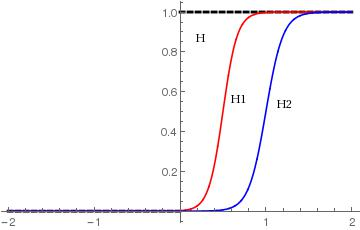
\includegraphics[width=2.5in]{fig2/heaviside.jpg}
\caption{\label{fig_heaviside}Plots of the Heaviside step function $H(x)$ (denoted by the black dashed line), and smoothed Heaviside step functions $H_1(x)$ (by the red solid line) and $H_2(x)$ (by the blue solid line). For the definitions of $H_1(x)$ and $H_2(x)$, see Eqs.~\eqref{H1} and \eqref{H2}.}
\end{figure}

By considerting two smoothed Heaviside step funstions
\begin{align}
\label{H1}
H_1(x)=\frac{1}{1+\mathrm{exp}(-12(x-\frac{1}{2}))},\\
\label{H2}
H_2(x)=\frac{1}{1+\mathrm{exp}(-10(x-1))},
\end{align}
the following arithmetic-mean average types are proposed:
\begin{equation}
\tilde{n}_\mathrm{arith}^{\mathrm{smooth},i} = \frac{1}{2}(n_1+n_2)H_i(\mathrm{min}(n_1,n_2)\Delta V),\quad (i=1,2).
\end{equation}
Note that the argument $x$ in $H_1(x)$ and $H_2(x)$ is not the number density $n$ but the number of particles in a cell, $n\Delta V$.
For the shape of these functions, see Fig.~\ref{fig_heaviside}.
Since $H_1(0)\approx 0$, $H_1(1/2)=1/2$, and $H_1(1)\approx 1$, it holds that $\tilde{n}_\mathrm{arith}^{\mathrm{smooth},1}\approx \tilde{n}_\mathrm{arith}$ unless the lower density cell has a fractional number of particles between 0 and 1.   
Similarly, from $H_2(0)\approx 0$, $H_2(1)=1/2$, and $H_2(2)\approx 1$, it holds that $\tilde{n}_\mathrm{arith}^{\mathrm{smooth},2}\approx \tilde{n}_\mathrm{arith}$ unless the lower density cell has a fractional number of particles between 0 and 2.   

\section{Results}

\begin{figure}
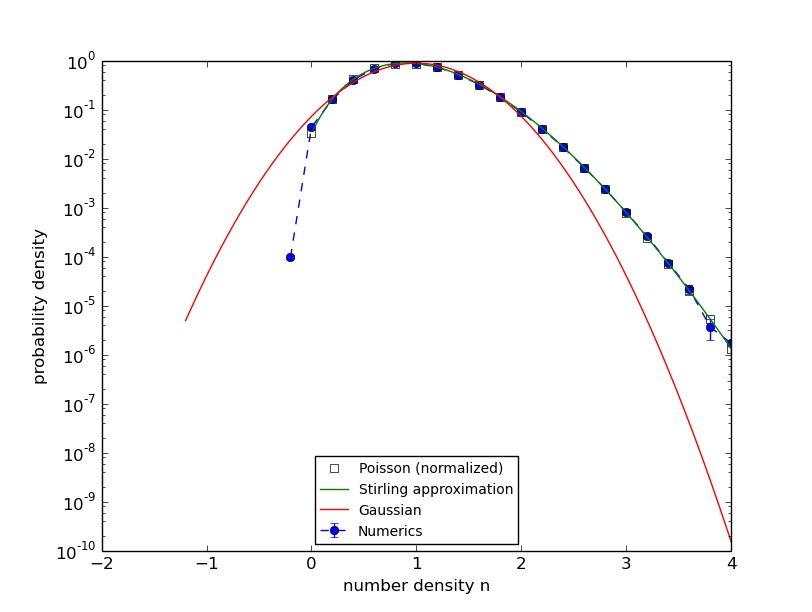
\includegraphics[width=0.5\linewidth]{fig2/hist_avg4.jpg}
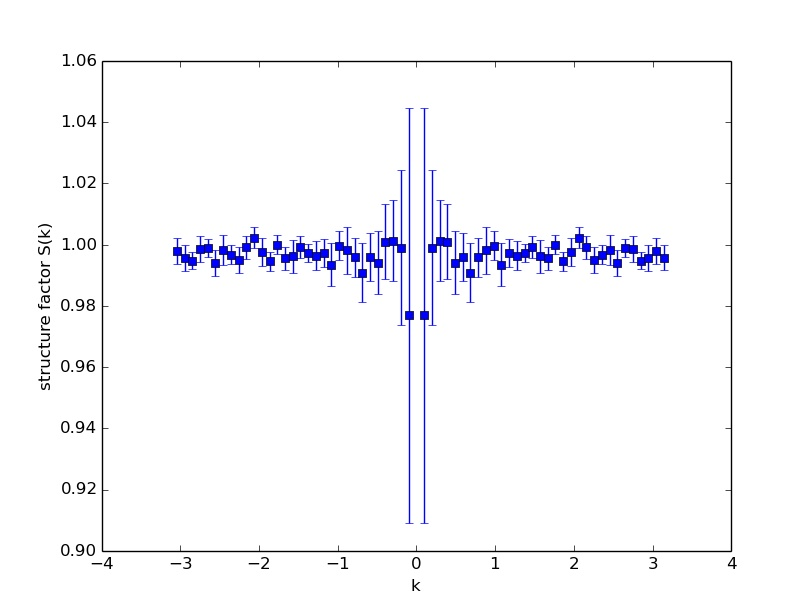
\includegraphics[width=0.5\linewidth]{fig2/Sk_avg4.jpg}
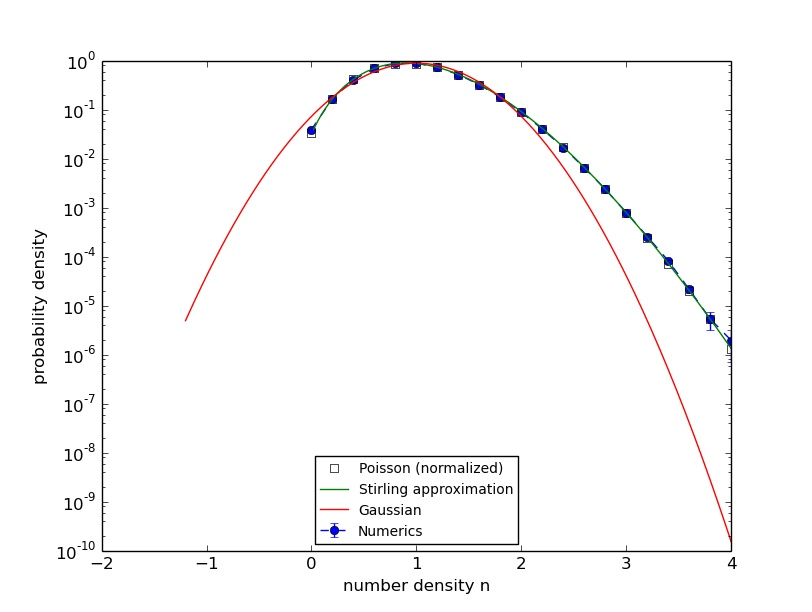
\includegraphics[width=0.5\linewidth]{fig2/hist_avg5.jpg}
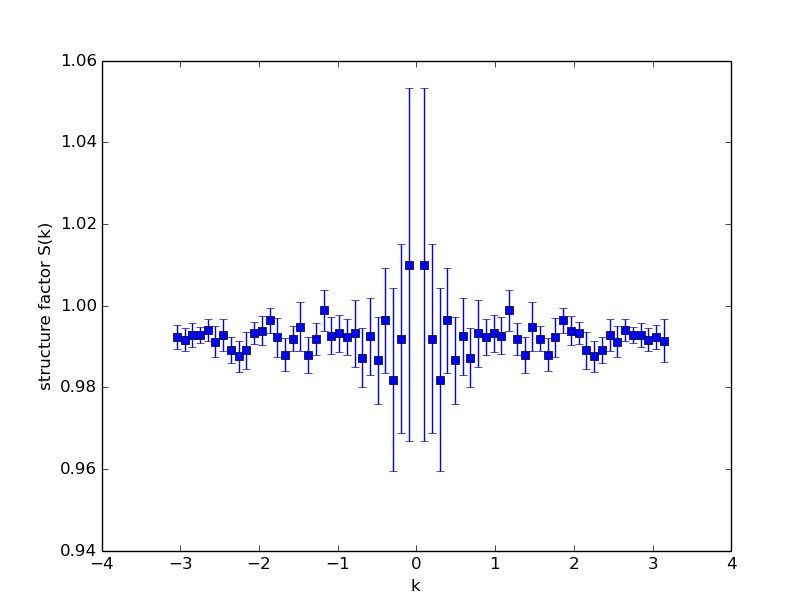
\includegraphics[width=0.5\linewidth]{fig2/Sk_avg5.jpg}
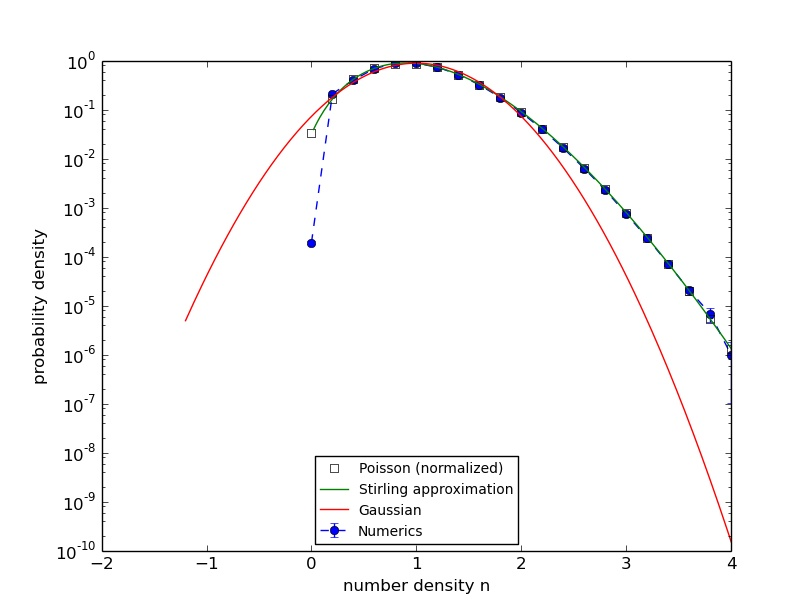
\includegraphics[width=0.5\linewidth]{fig2/hist_avg6.jpg}
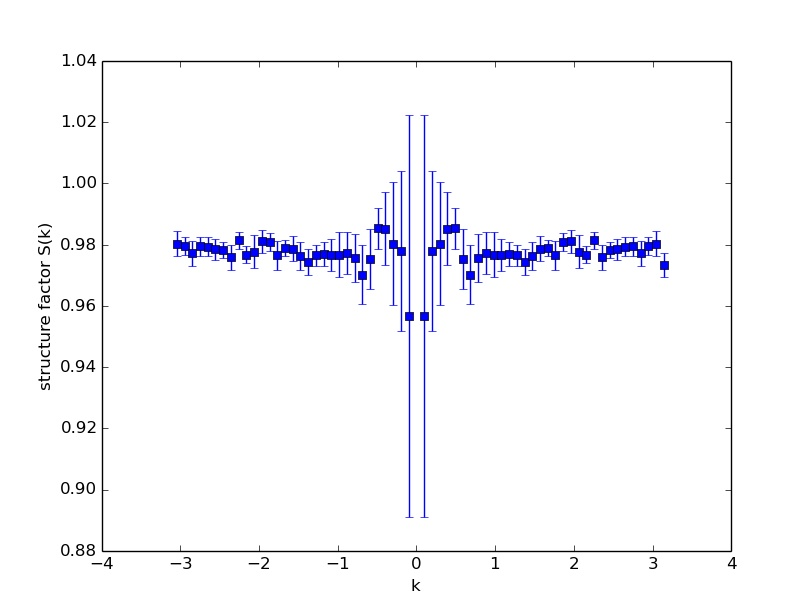
\includegraphics[width=0.5\linewidth]{fig2/Sk_avg6.jpg}
\caption{\label{fig_diff_456}[Diffusion-only case] Results of $\rho(n)$ (left column) and $S(k)$ (right column) for $\tilde{n}_\mathrm{arith}$ (arithmetic mean with Heaviside step function $H$, top row), $\tilde{n}_\mathrm{arith}^{\mathrm{smooth},1}$ (arithmetic mean with smoothed Heaviside step function $H_1$, middle row), and $\tilde{n}_\mathrm{arith}^{\mathrm{smooth},2}$ (arithmetic mean with smoothed Heaviside step function $H_2$, bottom row).
}
\end{figure}

\begin{figure}
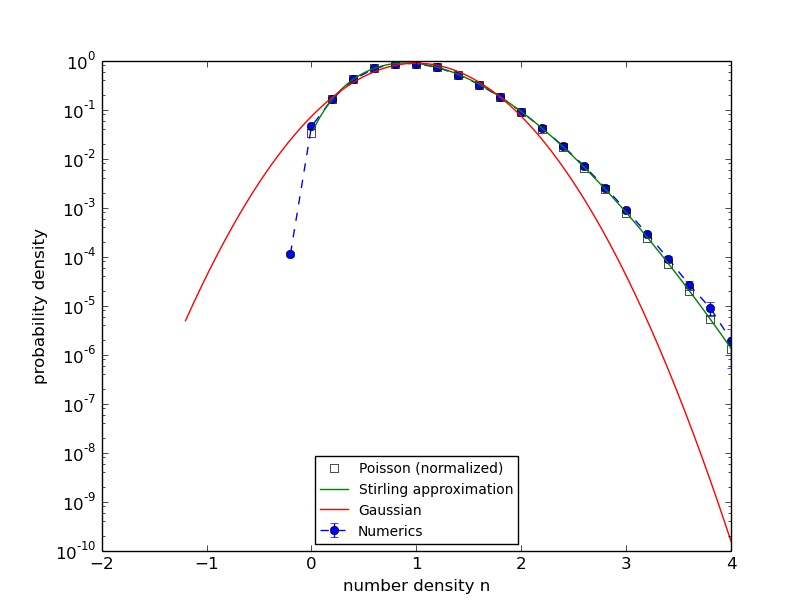
\includegraphics[width=0.5\linewidth]{fig2/react_hist_avg4.jpg}
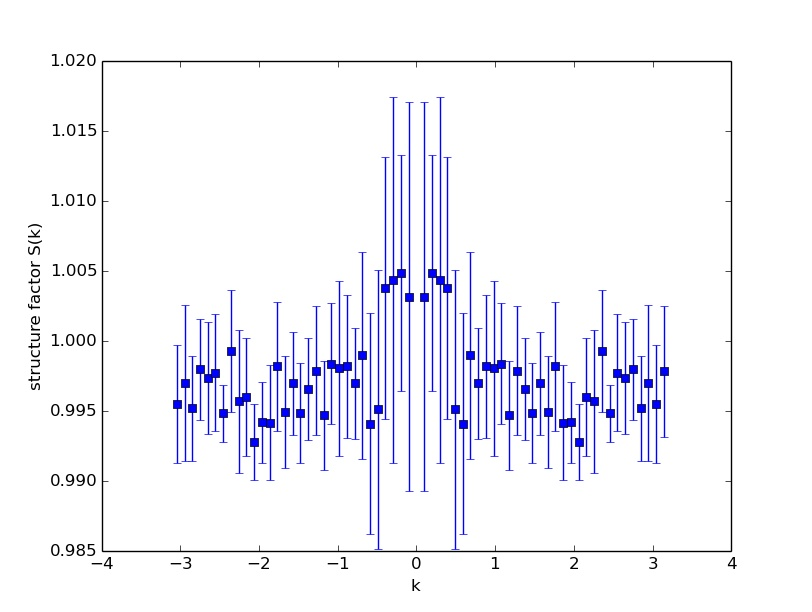
\includegraphics[width=0.5\linewidth]{fig2/react_Sk_avg4.jpg}
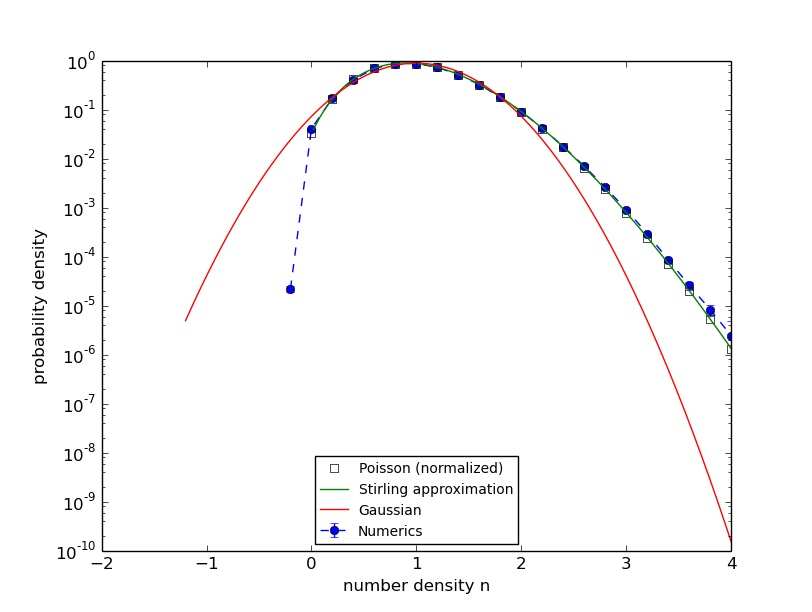
\includegraphics[width=0.5\linewidth]{fig2/react_hist_avg5.jpg}
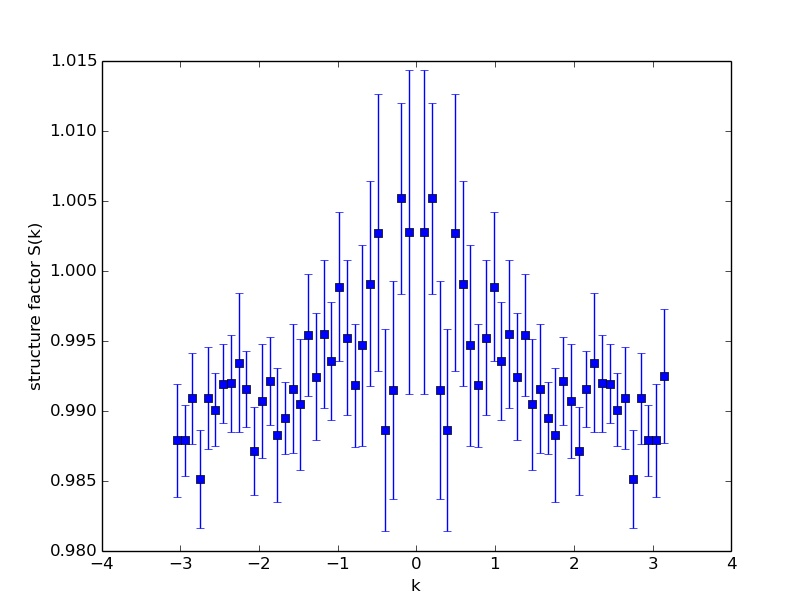
\includegraphics[width=0.5\linewidth]{fig2/react_Sk_avg5.jpg}
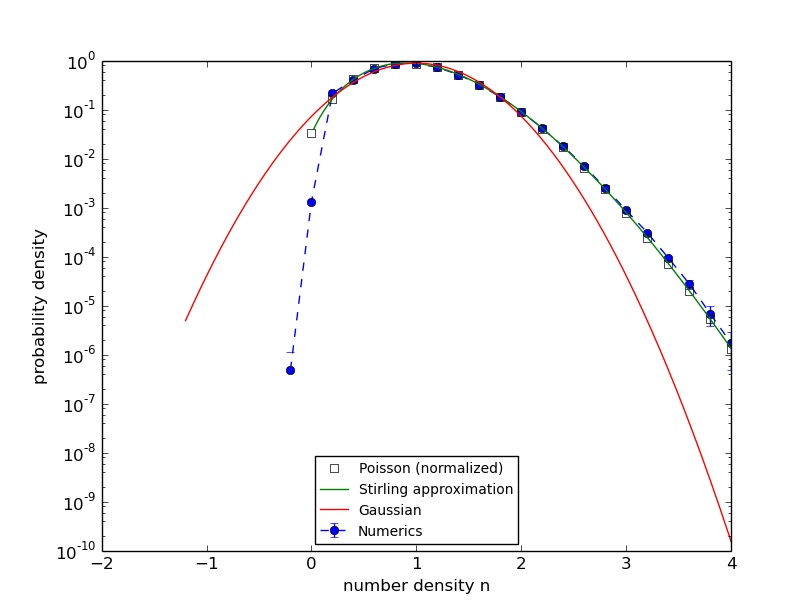
\includegraphics[width=0.5\linewidth]{fig2/react_hist_avg6.jpg}
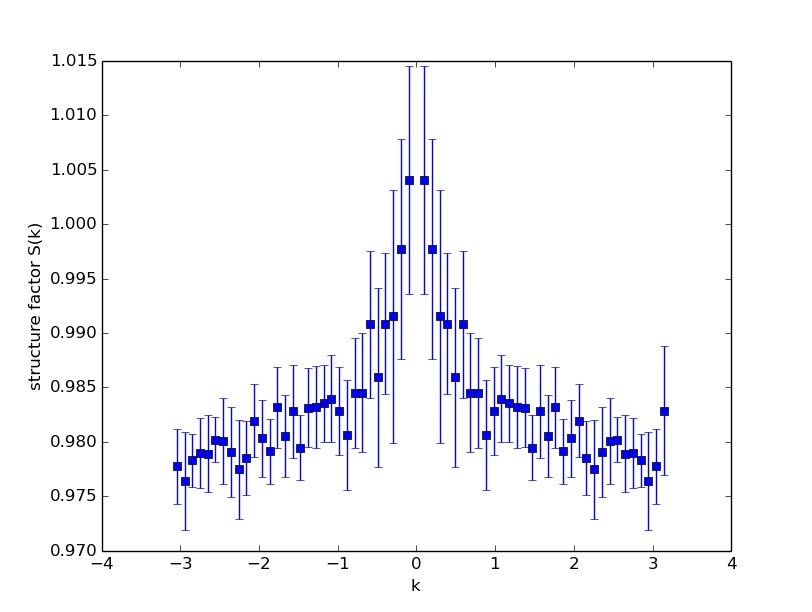
\includegraphics[width=0.5\linewidth]{fig2/react_Sk_avg6.jpg}
\caption{\label{fig_react_456}[Reaction-diffusion case] Results of $\rho(n)$ (left column) and $S(k)$ (right column) for $\tilde{n}_\mathrm{arith}$ (arithmetic mean with Heaviside step function $H$, top row), $\tilde{n}_\mathrm{arith}^{\mathrm{smooth},1}$ (arithmetic mean with smoothed Heaviside step function $H_1$, middle row), and $\tilde{n}_\mathrm{arith}^{\mathrm{smooth},2}$ (arithmetic mean with smoothed Heaviside step function $H_2$, bottom row).
}
\end{figure}

For the diffusion-only system, the number density distribution $\rho(n)$ and the structure factor $S(k)$ obtained from the three average types are shown in Fig.~\ref{fig_diff_456}.
The corresponding results to the reaction-diffusion system are shown in Fig.~\ref{fig_react_456}.
The values of $\mathrm{Var}[n]$ are as follows:
\begin{center}
{\tabulinesep=1.2mm
\begin{tabu}{|c|c|c|}
\hline
\multirow{2}{*}{Average type} & \multicolumn{2}{c|}{$\mathrm{Var}[n]$ (standard error)} \\
\cline{2-3}
 & Diffusion-only & Reaction-diffusion \\
\hline
$\tilde{n}_\mathrm{arith}$ & 0.1962 (0.0002) & 0.1994 (0.0001) \\
\hline
$\tilde{n}_\mathrm{arith}^{\mathrm{smooth},1}$ & 0.1954 (0.0002) & 0.1985 (0.0001) \\
\hline
$\tilde{n}_\mathrm{arith}^{\mathrm{smooth},2}$ & 0.1924 (0.0002) & 0.1967 (0.0001)\\
\hline
\end{tabu}
}
\end{center}

\paragraph{\textbf{Negative densities.}}
In the diffusion-only case, contrary to $\tilde{n}_\mathrm{arith}$, both $\tilde{n}_\mathrm{arith}^{\mathrm{smooth},1}$ and $\tilde{n}_\mathrm{arith}^{\mathrm{smooth},2}$ do not exhibit negative densities.
In the reaction-diffusion case, although all three average types allow nengative densities, chances of having negative densities are smaller in $\tilde{n}_\mathrm{arith}^{\mathrm{smooth},1}$ and even smaller in $\tilde{n}_\mathrm{arith}^{\mathrm{smooth},2}$.

\paragraph{\textbf{Density distribution value at $n=0$.}}
In both diffusion-only and reation-diffusion cases, the value of $\rho(0)$ is significantly different from the theoretical value for $\tilde{n}_\mathrm{arith}^{\mathrm{smooth},2}$.

\paragraph{\textbf{Structure factor and the variance}}
In the diffusion-only case, the flat value of $S(k)$ becomes smaller in $\tilde{n}_\mathrm{arith}^{\mathrm{smooth},1}$ and even smaller in $\tilde{n}_\mathrm{arith}^{\mathrm{smooth},2}$.
In the reaction-diffusion case, the shape of $S(k)$ is not flat any more and the overall values become smaller in these average types.
Correspondingly, the variance becomes smaller for these average types in both cases.

\section{Interpretations}

The observations made in the previous section have a tendency across the three average types and this can be explained by the following relation:
\begin{equation}
\tilde{n}_\mathrm{arith} \ge \tilde{n}_\mathrm{arith}^{\mathrm{smooth},1} \ge \tilde{n}_\mathrm{arith}^{\mathrm{smooth},2}.
\end{equation}
This relation is obtained from $H(x)\ge H_1(x)\ge H_2(x)$, see Fig.~\ref{fig_heaviside}.
The smaller variance of $n$ can be explained from the smaller noise intensity.
On the other hand, the smaller probability of negative densities can be explained as follows.
By replacing $H(x)$ with $H_1(x)$ or $H_2(x)$, noise intensity is significantly decreased when the two cells have very small number of particles.
This can prevent the cells from having negative densities.
However, it is noted that this artificial treatment causes physical quantities to deviate from theoretical predicitions.
The use of $H_2(x)$ significantly reduces the chances of having negative densities by reducing the noise intensity when the lower density cell has $\approx 1$ particle.
But, the value of $\rho(0)$ turns out to be much smaller than the theoretical value. 
 
The tentative conclusion for the best average type seems $\tilde{n}_\mathrm{arith}^{\mathrm{smooth},1}$.
Although the variance of $n$ and the overall values of $S(k)$ are slightly reduced, the chances for negative densities are significantly reduced in the diffusion-only case.
(Note that in the reaction-diffusion case, the tau-leaping method for the reaction part is another source of negative densities.)
It is noted that $H(x)\approx H_1(x)$ for any integer $x$.
By changing values for $0<x<1$, the issue of unphysical negative densities is somewhat resolved.
But, by not changing values for integer values of $x$, physical quantities are not significantly changed.

\section*{Appendix: Computational time}

Compared with $\tilde{n}_\mathrm{arith}$, calculating $\tilde{n}_\mathrm{arith}^{\mathrm{smooth,1}}$ may take more time due to the evaluation of the exponential function in $H_1(x)$. 
By considering that $1-H_1(x)<4\times10^{-11}$ for $x>2.5$, the evaluation of the exponential function may be avoided for $x>2.5$ by simply assigning $H_1(x)=1$.
This is very effective when cells have a large number of particles.

These predictions have been confirmed by comparing the computational time spent in \texttt{average\_to\_faces} routine.
$\tilde{n}_\mathrm{arith}$ and  $\tilde{n}_\mathrm{arith}^{\mathrm{smooth,1}}$ are implemented by options \texttt{avg\_type=4} and \texttt{5}.
The modified version of $\tilde{n}_\mathrm{arith}^{\mathrm{smooth,1}}$ is implemented by \texttt{avg\_type=7}.
The computational times for average number of particles in a cell $N=5$ and 100 are as follows:
\begin{center}
{\tabulinesep=1.2mm
\begin{tabu}{|c|c|c|}
\hline
\multirow{2}{*}{\texttt{avg\_type}} & \multicolumn{2}{c|}{time (ms)} \\
\cline{2-3}
 & $N=5$ & $N=100$ \\
\hline
\texttt{4} & 1350 & 1352 \\
\hline
\texttt{5} & 2504 & 4780 \\
\hline
\texttt{7} & 1780 & 1511 \\
\hline
\end{tabu}
}
\end{center}
As expected, for the large-number-of-particle-in-a-cell case, \texttt{avg\_type=7} is much faster than \texttt{avg\_type=5} and rather comparable to \texttt{avg\_type=4}.

\end{document}
